% Where the hand ends up: the error terms, and the 30 mm gate they must fit in.
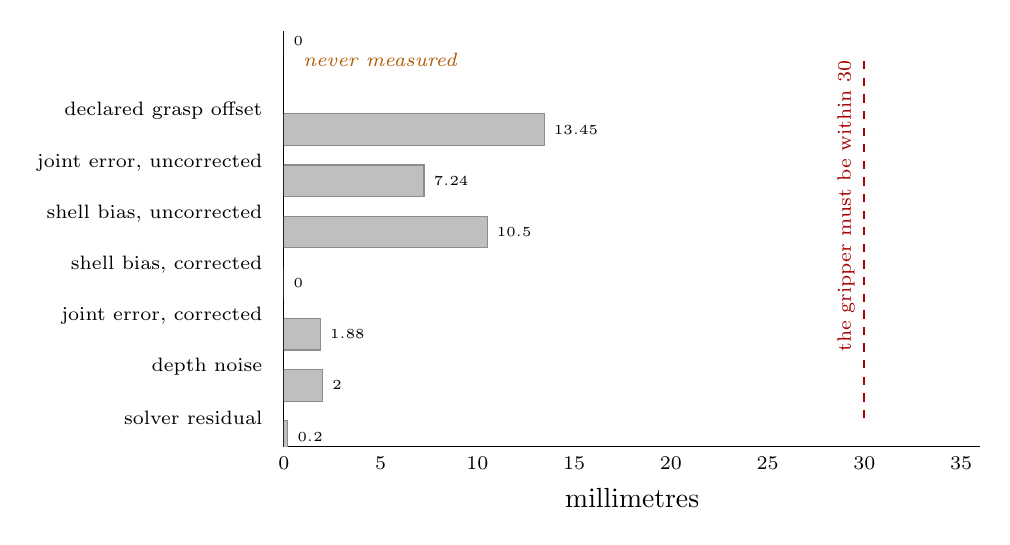
\begin{tikzpicture}
\begin{axis}[
    width=0.86\linewidth, height=58mm,
    xbar, y=6.5mm, bar width=4mm,
    xmin=0, xmax=36,
    xlabel={millimetres},
    symbolic y coords={
      {solver residual},
      {depth noise},
      {joint error, corrected},
      {shell bias, corrected},
      {shell bias, uncorrected},
      {joint error, uncorrected},
      {declared grasp offset},
      {camera mounting}},
    ytick=data,
    y tick label style={font=\scriptsize},
    x tick label style={font=\scriptsize},
    nodes near coords, nodes near coords style={font=\tiny},
    every node near coord/.append style={anchor=west},
    enlarge y limits=0.08,
    axis lines*=left,
    tick style={draw=none},
]
\addplot[fill=black!25, draw=black!45] coordinates {
  (0.2,{solver residual})
  (2.0,{depth noise})
  (1.88,{joint error, corrected})
  (0.0,{shell bias, corrected})
  (10.5,{shell bias, uncorrected})
  (7.24,{joint error, uncorrected})
  (13.45,{declared grasp offset})
};
\addplot[fill=orange!45, draw=orange!70!black] coordinates {
  (0,{camera mounting})
};
\node[font=\scriptsize\itshape, anchor=west, orange!70!black]
  at (axis cs:0.5,{camera mounting}) {never measured};
\draw[red!65!black, thick, dashed]
  (axis cs:30,{solver residual}) -- (axis cs:30,{camera mounting});
\node[font=\scriptsize, red!65!black, anchor=south, rotate=90]
  at (axis cs:30,{shell bias, uncorrected}) {\ \ the gripper must be within \SI{30}{\milli\metre}};
\end{axis}
\end{tikzpicture}
